\documentclass[11pt,oneside,openany]{book}

\usepackage[a4paper,margin=25mm]{geometry}
\usepackage{cscover}
\usepackage[dvipdfmx]{graphicx}
\usepackage[nobreak]{cite}
\usepackage[a4paper,dvipdfmx,pdfdisplaydoctitle=true,%
    bookmarks=true,bookmarksnumbered=true,bookmarkstype=toc,bookmarksopen=true,%
    pdftitle={A Study on Thesis Formats},%
    pdfauthor={Author Name}%
    ]{hyperref}

\usepackage[cmex10]{amsmath}
\usepackage{amssymb,amsfonts}
\interdisplaylinepenalty=2500
\usepackage{dblfloatfix}
\usepackage{booktabs}
\usepackage{siunitx}
\usepackage[numbers,compress]{natbib}
\usepackage{texnames}
\usepackage{bm,bbm}
\usepackage{orcidlink}
\usepackage{latexsym}
\usepackage{array}
\usepackage{mathtools}
\usepackage{caption}
\usepackage{subcaption}
\usepackage{multirow}
\usepackage{multicol}
\usepackage{setspace}
\usepackage{algorithm}
\usepackage{algpseudocode}

\renewcommand{\bibname}{References}
\pagestyle{plain}

\thesistype{Independent Research Project Report:\\Bachelor's Thesis}
\title{Efficient and Accurate Full-Waveform Inversion with Total Variation Constraint}
\author{Yudai INADA, Shingo TAKEMOTO, and Shunsuke ONO}
\studentid{21B39015}
\affiliation{%
  Department of Computer Science\\
  School of Computing\\
  Institute of Science Tokyo}
\date{January, 2025}

\supervisorname{Supervisor:}
\supervisor{Shunsuke ONO}
%\dsupervisorname{Deputy Supervisor:}
%\dsupervisor{Jiro Kogaku}

% vec
\newcommand{\vecx}{\bm{x}}
\newcommand{\vecy}{\bm{y}}

% utils
\newcommand{\argmax}[1]{\underset{#1}{\mathrm{argmax}}}
\newcommand{\argmin}[1]{\underset{#1}{\mathrm{argmin}}}
\newcommand{\minimize}[1]{\underset{#1}{\mathrm{min}}}
\newcommand{\maximize}[1]{\underset{#1}{\mathrm{min}}}
\newcommand{\Norm}[2]{\lVert #1 \rVert}
\newcommand{\LOneNorm}[1]{\lVert #1 \rVert _1}
\newcommand{\LTwoNorm}[1]{\lVert #1 \rVert _2}
\newcommand{\LOneTwoNorm}[1]{\lVert #1 \rVert _{1,2}}
\newcommand{\TV}[1]{\mathrm{TV}(#1)}
\newcommand{\realNumber}{\mathbb{R}}
\newcommand{\intN}{\mathrm{N}}
\newcommand{\intM}{\mathrm{M}}

\newcommand{\LOneTwoNormDefinition}{\LOneTwoNorm{\vecx} \coloneq  \sum_{\mathfrak{g} \in \mathfrak{G}} \LTwoNorm{\vecx_\mathfrak{g}}}
\newcommand{\TotalVariationDefinition}{\TV{\vecx} \coloneq \LOneTwoNorm{\diffOperator \vecx} = \sum_{i=1}^{\intN} \sqrt{d_{h,i}^2 + d_{v,i}^2}}
\newcommand{\conjugateFunctionDefinition}{f^*(\vecx) \coloneq \sup_{\vecy \in \realNumber^N} \left\{ \vecy^T \vecx - f(\vecy) \right\}}

% indicator function
\newcommand{\indicatorFunction}[2]{\iota_{#1}(#2)}
\newcommand{\indicatorFunctionDefinition}{\indicatorFunction{C}{\vecx} \coloneq \begin{cases} 0 & \text{if } \vecx \in C, \\ \infty & \text{otherwise}. \end{cases} }

% proximity operator
\newcommand{\proximityOperator}[2]{\mathrm{prox}_{#1}\left(#2\right)}
\newcommand{\proximityOperatorDefinition}{\proximityOperator{ \gamma f }{\vecx} := \argmin{\vecy \in \realNumber^N} \left\{ f(\vecy) + \frac{1}{2 \gamma} \LTwoNorm{\vecy - \vecx}^2 \right\}}
\newcommand{\proximityOperatorDefinitionWithConvexConjugateFunction}{\proximityOperator{ \gamma f^* }{\vecx} = \vecx - \gamma \proximityOperator{ \frac 1 \gamma f }{\frac 1 \gamma \vecx} }
\newcommand{\projBox}[1]{ P_{[a,b]^N}(#1) }
\newcommand{\projBoxSolution}{ \projBox{\vecx} = \text{min}( \text{max} (\vecx, a), b) }
\newcommand{\projLOneTwoBall}[1]{P_{ \{ \LOneTwoNorm{ \cdot } \le \alpha \} }(#1)}
\newcommand{\projLOneTwoBallSolution}{
    (\projLOneTwoBall{\vecx})_{\mathfrak{g}_i} =
        \begin{cases}
            0 & \text{if} \ \LTwoNorm{\vecx_{\mathfrak{g}_i}} = 0, \\
            \bm \beta_i \frac {\vecx_{\mathfrak{g}_i}} {\LTwoNorm{\vecx_{\mathfrak{g}_i}}} & \text{otherwise},
        \end{cases} \\
}
\newcommand{\projLOneTwoBallSolutionWhere}{
    \bm \beta = P_{ \{ \LOneNorm{ \cdot } \le \alpha \} }({[ \LTwoNorm{ \vecx_{\mathfrak{g}_1} }, \ldots, \LTwoNorm{ \vecx_{\mathfrak{g}_N} } ]^T}). \\
}
\newcommand{\projLOneBall}[1]{P_{ \{ \LOneNorm{ \cdot } \le \alpha \} }(#1)}
\newcommand{\projLOneBallSolution}{\projLOneBall{\vecx} = \text{SoftThrethold}(\vecx, \beta)}
\newcommand{\projLOneBallSolutionWhere}{
    \begin{aligned}
        & \bm x_{\text{abs}} = \text{abs}(\vecx), \\
        & \bm y              = \text{sort}_{\text{desc}}(\vecx_{\text{abs}}), \\
        & \beta'             = \text{max} \{ \frac 1 i ((\sum_{j=1}^i \bm y_j) - \alpha) \mid i = 1, \ldots, N \}, \\
        & \beta              = \text{max} \{ \beta', 0 \}. \\
    \end{aligned}
}


% Primal-Dual Splitting
\newcommand{\PDSPrimal}{\minimize { \vecx \in \realNumber^N } \left\{ f(\vecx) + g(\vecx) + h(\bm{L} \vecx) \right\} }
\newcommand{\PDSDual}{\minimize { \vecy \in \realNumber^M } \left\{ (f+g)^*(-\bm{L}^T \vecy) + h^*(\vecy) \right\} }
\newcommand{\PDSSubStep}{
\left \lfloor \ \
    \begin{aligned}
        & \vecx^{(k+1)} = \proximityOperator{\gamma_1 g}{\vecx^{(k)} - \gamma_1( \nabla f(\vecx^{(k)}) + \bm{L}^T \vecy^{(k)} )}, \\
        & \vecy^{(k+1)} = \proximityOperator{\gamma_2 h^*}{\vecy^{(k)} + \gamma_2 \bm{L} (2\vecx^{(k+1)} - \vecx^{(k)}) }, \\
    \end{aligned}
\right.
}

% seismic + related proposed method
\newcommand{\diffOperator}{\mathbf{D}}
\newcommand{\velModel}{\bm{m}}
\newcommand{\seismicData}{\bm{u}}

% FWI objective
\newcommand{\FWIObjectiveDefinition}{ E(\velModel) = \frac {1} {2} \LTwoNorm { \seismicData_{\mathrm{obs}} - \seismicData_{\mathrm{cal}}(\velModel) }^2 }
\newcommand{\FWIGradientDefinition}{ \nabla E(\velModel) = \seismicData_{\mathrm{obs}} - \nabla \seismicData_{\mathrm{cal}(\velModel)} }
\newcommand{\FWIObjectiveWithTVConstraint}{ E(\velModel) \ \ \ \text{s.t.} \ \ \LOneTwoNorm{\diffOperator \velModel} \le \alpha \ , \ \velModel \in [a,b]^N }
\newcommand{\FWIObjectiveWithTVConstraintWithIndicatorFunction}{ E(\velModel) + \indicatorFunction{\LOneTwoNorm{\cdot} \le \alpha}{\diffOperator \velModel} + \indicatorFunction{[a,b]^N}{\velModel} }
\newcommand{\FWIWithPDS}{
\left \lfloor \ \
    \begin{aligned}
        & \widetilde{\velModel}^{(k+1)} = \velModel^{(k)} - \gamma_1( \nabla E(\velModel^{(k)}) + \bm{D}^T \vecy^{(k)} ) \\
        & \velModel^{(k+1)}             = \projBox{\widetilde{\velModel}^{(k+1)}} \\
        & \widetilde{\vecy}^{(k+1)}     = \vecy^{(k)} + \gamma_2 \bm{D} (2\velModel^{(k+1)} - \velModel^{(k)}) \\
        & \vecy^{(k+1)}                 = \widetilde{\vecy}^{(k+1)} - \gamma_2 \projLOneTwoBall{\frac 1 {\gamma_2} {\widetilde{\bm y}^{(k+1)}}}
    \end{aligned}
\right.
}
\newcommand{\FWIWithGradient}{ \velModel^{(k+1)} = \velModel^{(k)} - \gamma( \nabla E(\velModel^{(k)}) ) }





\begin{document}
    \makeatletter
\def\bstctlcite{\@ifnextchar[{\@bstctlcite}{\@bstctlcite[@auxout]}}
\def\@bstctlcite[#1]#2{\@bsphack
\@for\@citeb:=#2\do{%
\edef\@citeb{\expandafter\@firstofone\@citeb}%
\if@filesw\immediate\write\csname #1\endcsname{\string\citation{\@citeb}}\fi}%
\@esphack}
\makeatother
\bstctlcite{IEEEexample:BSTcontrol}


    \frontmatter
    \maketitle

    \chapter{Abstract} \label{ch:abstract}  \input{src/0-abstract}

    \tableofcontents
    \listoffigures
    \listoftables

    %%%%%%%%%%%%%%%%%%%%%%%%%%%%%%%%%%%%%%%%%%%%%%%%%%

    \mainmatter

    \chapter{Introduction}    \label{ch:introduction}   Full waveform inversion (FWI)~\cite{FWI0,FWI1} aims to reconstruct subsurface properties from observed seismic data.
These properties are used for geological research and resource exploration, including gas, oil, mineral deposits and groundwater~\cite{FWI1,FWIApplicationGroundwater0,FWIApplicationGroundwater1}.
FWI has also been applied to non-destructive testing~\cite{FWIApplicationNonDestructiveTesting0,FWIApplicationNonDestructiveTesting1}.

Since the observed seismic data are generated by subsurface properties, FWI is formulated as an inverse problem.
However, it is ill-posed, and the quality of the solution depends significantly on the initial model~\cite{FWI1}.
To achieve accurate reconstruction, several formulations have been proposed~\cite{FWI0,CustomFWI0,CustomFWI1,CustomFWI2,CustomFWI3,CustomFWI4,CustomFWI5}.
Typically, FWI is treated as an optimization problem, where the objective is to minimize the squared error between observed and modeled data.

To enhance stability and accuracy, regularization terms are often added to the objective function, such as Tikhonov regularization~\cite{tikhonov}, Total Variation (TV)~\cite{TV}, and Total Generalized Variation (TGV)~\cite{TGV}.
For example, studies have used regularization of Tikhonov~\cite{FWI-with-tikhonov-regularization}, TV~\cite{FWI-with-TV-regularization}, directional TV~\cite{FWI-with-directional-TV-regularization}, high-order TV~\cite{FWI-with-high-order-TV-regularization}, and TGV~\cite{FWI-with-TGV-regularization}.

The value of the objective function of FWI depends on the observation method, because it contains the squared error between the observed data and the modeled data.
Consequently, the regularization parameters must be adapted to the observation method.
While, adding constraints to the objective function is advantageous because their parameters can be derived only from prior knowledge of the subsurface properties~\cite{constraints-vs-penalties-in-FWI}.
Therefore, it has been proposed to add the TV constraint to the objective function~\cite{FWI-with-TV-constraint,FWI-with-TV-constraint2,FWI-with-TV-constraint3}.

In conventional methods that apply the TV constraint to FWI~\cite{FWI-with-TV-constraint,FWI-with-TV-constraint2}, parameter updates in optimization algorithms are adjusted to satisfy the constraints.
This often requires an additional optimization step, resulting in an inner loop and increased computational cost.
In addition, approximations are introduced to incorporate constraints, such as treating non-linear transformations as linear or imposing constraints outside the optimization method.

In this paper, we develop an efficient algorithm based on a primal-dual splitting method to solve the TV-constrained FWI problem with neither an inner loop nor approximations.
...嬉しさを詳細に書く.
We also demonstrate the effectiveness of the proposed method through experiments using the SEG/EAGE Salt and Overthrust Models.




    \chapter{Preliminaries}   \label{ch:preliminaries}  \subsection{Mathematical Tools}\label{subsec:mathematical-tools}

Throughout this paper, we denote vector and matrix by bold lowercase letters (e.g., $\vecx$) and bold uppercase letters (e.g., $\bm{X}$), respectively.
The operator $l_{X}$ norm of a vector and matrix is denoted by $\Norm{\cdot}__{X}$.

For $\vecx \in \realNumber^{\intN}$, the mixed $l_{1,2}$ norm is defined as follows:
\begin{equation} \label{eq:L12NormDefinitionEq} \LOneTwoNormDefinition, \end{equation}
where $\mathfrak{G}$ is a set of disjoint index sets, and $\vecx_{\mathfrak{g}}$ is the subvector of $\vecx$ indexed by $\mathfrak{g}$.

For $\vecx \in \realNumber^{\intN}$, the total variation (TV)~\cite{TV} is defined as follows:
\begin{equation} \label{eq:TVDefinitionEq} \TotalVariationDefinition, \end{equation}
where $d_{h,i}$ and $d_{v,i}$ are the horizontal and vertical differences of the $i$-th element of $\vecx$, respectively, when the vector $\vecx$ is considered as a matrix.

For a proper lower-semicontinuous convex function $f \in \realNumber^N \to \realNumber$ and $\vecx \in \realNumber^N$, the convex conjugate function is defined as follows:
\begin{equation} \label{eq:ConjugateFunctionDefinitionEq} \conjugateFunctionDefinition. \end{equation}

For a set $C \subset \realNumber^N$ and $\vecx \in \realNumber^N$, the indicator function is defined as follows:
\begin{equation} \label{eq:IndicatorFunctionDefinitionEq} \indicatorFunctionDefinition \end{equation}

For $\gamma > 0$, $f \in \realNumber^N \to \realNumber$ and $\vecx \in \realNumber^N$, the proximity operator is defined as follows:
\begin{equation} \label{eq:ProximityOperatorDefinitionEq} \proximityOperatorDefinition. \end{equation}

Define the proximity operator for the indicator function as $P_C$ as follows.
\begin{equation} \label{eq:ProximityOperatorDefinitionWithIndicatorFunctionEq}
\proximityOperator{ \gamma \indicatorFunction{C}{\cdot} }{\vecx} = P_C(\vecx) \coloneq \argmin{\vecy \in C} \LTwoNorm{\vecy - \vecx}.
\end{equation}

%Below is the proximity operator for the specific function used in this paper.
The proximity operator for the convex conjugate function is expressed as follows~\cite[Theorem 3.1 (ii)]{prox-convex-conjugate-function}:
\begin{equation} \label{eq:ProximityOperatorDefinitionWithConvexConjugateFunctionEq} \proximityOperatorDefinitionWithConvexConjugateFunction. \end{equation}

%The proximity operator for the box constraint is expressed as follows.

\subsection{Primal-Dual Splitting Algorithm}\label{subsec:primal-dual-splitting-algorithm}
The Primal-Dual Splitting (PDS) algorithm~\cite{PDS0,PDS1,PDS2,PDS3} is applied to the following problem:
\begin{equation} \label{eq:PDSPrimalEq} \PDSPrimal, \end{equation}
where $\bm{L} \in \realNumber^{\intM \times \intN}$, $f$ is a differentiable convex function and $g,h$ are convex functions whose proximity operator can be computed efficiently.

The PDS algorithm solves by iteratively updating the following:
\begin{equation} \label{eq:PDSSubStep} \PDSSubStep \end{equation}
where $\gamma_1, \gamma_2 \in \realNumber$ are step sizes.


\begin{figure*}[htbp]
    \centering
    \begin{tabular}{m{144mm} m{10mm} m{0mm}}
        \begin{minipage}[b]{146mm}
            \centering
            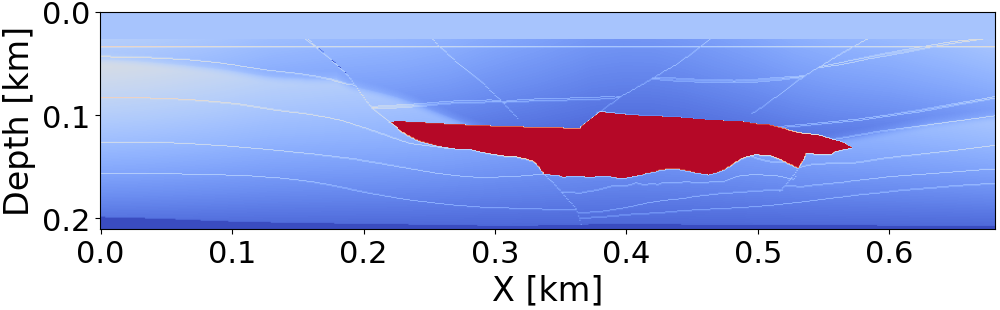
\includegraphics[width=146mm]{public/full_true_vm}
        \end{minipage} &
        \begin{minipage}[b]{20mm}
            \centering
            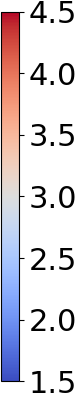
\includegraphics[height=49mm]{public/color-bar}
        \end{minipage} &
    \end{tabular}
    \caption{the velocity model of the Salt [km/s]}
    \label{fig:salt-model}
\end{figure*}



\subsection{Full Waveform Inversion}\label{subsec:full-waveform-inversion}
Typically, FWI is treated as an optimization problem as follows\cite{FWI0}:
\begin{equation} \label{eq:FWIObjective} \argmin{\velModel \in \realNumber^N} \ \ \FWIObjectiveDefinition, \end{equation}
where $\velModel \in \realNumber^{N}$ is the velocity model representing subsurface properties, $\seismicData_{\mathrm{obs}} \in \realNumber^{M}$ is the observed seismic data, $\seismicData_{\mathrm{cal}}$ is the observation process, and $\seismicData_{\mathrm{cal}(\velModel)}$ is the modeled seismic data with the velocity model.
$N$ is the number of grid points, and $M$ is the number of observed signals.
In general, the velocity model is 2D or 3D grid data, but for simplicity we consider flattened 1D vector.

The observation process is nonlinear and complex, making it difficult to obtain $\seismicData_{\mathrm{cal}(\cdot)}$ analytically.
However, the gradient $\nabla E$ can be computed numerically using the adjoint-state method~\cite{FWI-gradient}.

Therefore, the standard FWI minimizes the objective function and reconstructs the velocity model using the following procedures:
\begin{equation} \label{eq:FWIWithGradient} \FWIWithGradient, \end{equation}
where $\gamma$ is the step size.


    \chapter{Proposed Method} \label{ch:proposedmethod} We introduce the TV and box constraint into the FWI problem to achieve more accurate reconstruction.
As shown in Fig.~\ref{fig:salt-model}, the velocity model is piecewise smooth, thus introducing the TV constraint to achieve a more accurate reconstruction.
Also, by introducing the box constraint, we prevent the velocity model values from being invalid.
As mentioned in the introduction, it is easier to determine parameters if the TV is treated as a constraint rather than a regularization.

The optimization problem of the TV and box constrained FWI is formulated as follows:
\begin{equation} \label{eq:FWIObjectiveWithTVConstraint} \argmin{\velModel \in \realNumber^N} \ \ \FWIObjectiveWithTVConstraint \end{equation}
where $\alpha \in \realNumber$ is the upper bound of the $l_{1,2}$ norm, and $l, u \in \realNumber$ are the lower and upper bounds of the velocity model values, respectively.

The constraints can be incorporated into the objective function as indicator functions:
\begin{equation} \label{eq:FWIObjectiveWithTVConstraintWithIndicatorFunction} \argmin{\velModel \in \realNumber^N} \ \ \FWIObjectiveWithTVConstraintWithIndicatorFunction. \end{equation}

The proximity operator of $\iota_{\LOneTwoNorm{\cdot} \le \alpha}$ and $\iota_{[l,u]^N}$ can be computed efficiently.
Therefore, these functions of $E$, $\iota_{[l,u]^N}$ and $\iota_{\LOneTwoNorm{\cdot} \le \alpha}$ correspond to $f$, $g$ and $h$ in \eqref{eq:PDSPrimalEq}, respectively, $\diffOperator$ is corresponds to $\bm{L}$, so the problem~\eqref{eq:FWIObjectiveWithTVConstraintWithIndicatorFunction} can be solved using PDS.
We show the detailed algorithm in Algorithm~\ref{alg:FWIWithPDS}.
%\begin{equation} \label{eq:FWIWithPDS} \FWIWithPDS \notag \end{equation}
\begin{algorithm}[t]
    \caption{PDS for \eqref{eq:FWIObjectiveWithTVConstraintWithIndicatorFunction}}\label{alg:FWIWithPDS}
    \begin{algorithmic}[1]
        \Statex \textbf{Input:} $ \velModel^{(0)}, \vecy^{(0)}, \gamma_0 > 0, \gamma_1 > 0 $
        \While {A stopping criterion is not satisfied}
            \State $\widetilde{\velModel} \leftarrow \FWIWithPDSStepMTmp $
            \State $\velModel^{(k+1)}     \leftarrow \FWIWithPDSStepM $
            \State $\widetilde{\vecy}     \leftarrow \FWIWithPDSStepYTmp $
            \State $\vecy^{(k+1)}         \leftarrow \FWIWithPDSStepY $
        \EndWhile
        \Statex \textbf{Output:} $\velModel^{(k)}$
    \end{algorithmic}
\end{algorithm}


The proximity operators of $\iota_{[l,u]^N}$, $\iota_{\LOneTwoNorm{\cdot} \le \alpha}$, that is, the projection onto $[l,u]^N$ and ${\LOneTwoNorm{\cdot} \le \alpha}$ are calculated by
\begin{equation} \label{eq:ProximityOperatorForBoxConstraint} \projBoxSolution, \end{equation}

%The proximity operator for the $l_{1,2}$ norm upper bound constraint is expressed as follows~\cite{L12-ball-projection}:
\begin{equation} \label{eq:ProximityOperatorForL12Ball} \projLOneTwoBallSolution \end{equation}
where
\begin{equation} \label{eq:ProximityOperatorForL12BallWhere} \projLOneTwoBallSolutionWhere \notag \end{equation}

The proximity operator for the $l_1$ norm upper bound constraint is expressed as follows~\cite{L1-ball-projection}:
\begin{equation} \label{eq:ProximityOperatorForL1Ball}  \projLOneBallSolution, \end{equation}
where
\begin{equation} \label{eq:ProximityOperatorForL1BallWhere} \projLOneBallSolutionWhere \notag \end{equation}

The computation of $\nabla E$ requires the simulation of the wave equation along the time axis for each grid point.
In contrast, the computation of the other parts of the process can be done without time axis simulations.
Therefore, the computationally intensive part of the process is primarily the calculation of $\nabla E$, and the introduction of the constraints does not significantly increase the overall computational cost.

    \chapter{Experiments}     \label{ch:experiments}    

\begin{figure*}[htbp]
    \centering
    \begin{tabular}{m{68mm} m{70mm} m{10mm}}
        \begin{minipage}[b]{70mm}
            \centering
            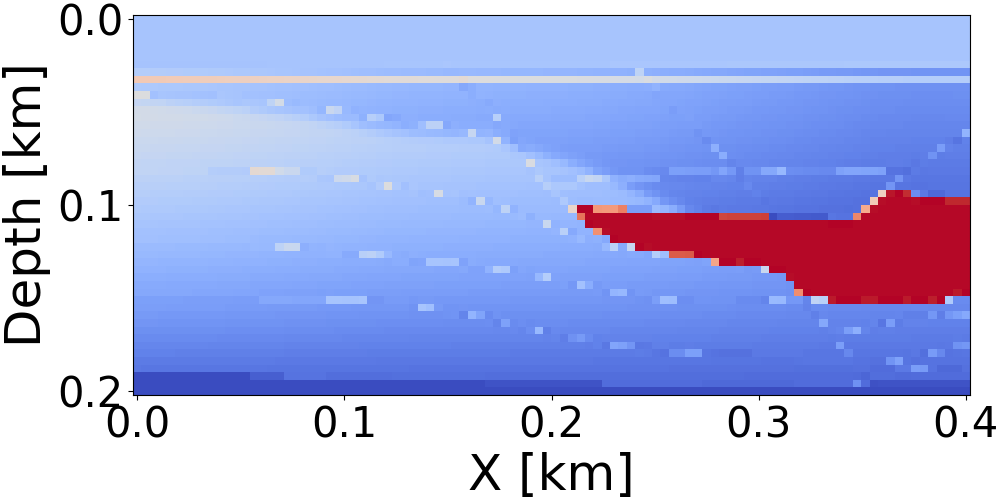
\includegraphics[width=70mm]{public/true}
            \vspace{-7mm}
            \caption*{\raisebox{2mm}{Background truth}}
        \end{minipage} &
        \begin{minipage}[b]{70mm}
            \centering
            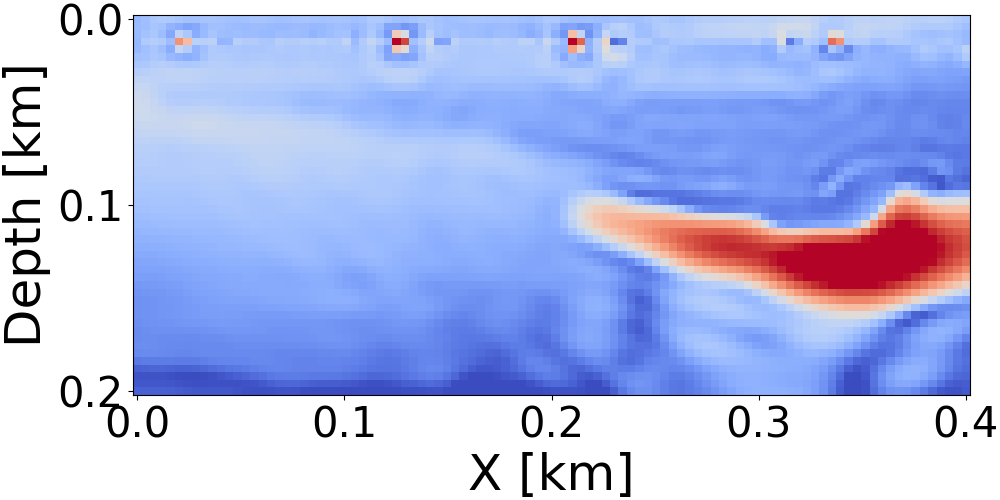
\includegraphics[width=70mm]{public/gradient}
            \vspace{-7mm}
            \caption*{\raisebox{2mm}{Reconstructed with standard FWI}}
        \end{minipage} &
        \multirow[t]{2}{*}{\raisebox{-50mm}{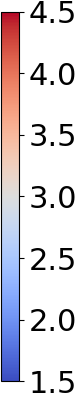
\includegraphics[height=68mm]{public/color-bar}}} \\
        \begin{minipage}[b]{70mm}
            \centering
            
\includegraphics[width=70mm]{public/initial}
            \vspace{-8mm}
            \caption*{Initial model}
        \end{minipage} &
        \begin{minipage}[b]{70mm}
            \centering
            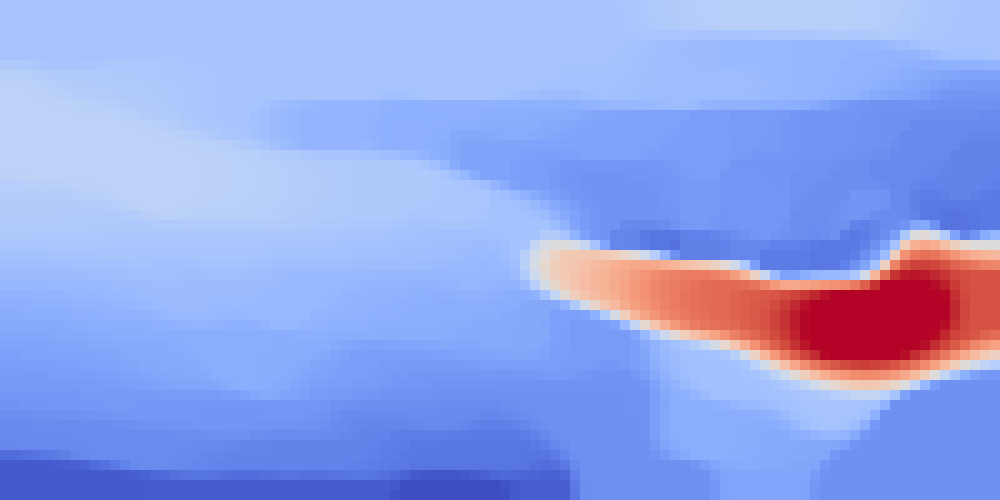
\includegraphics[width=70mm]{public/pds}
            \vspace{-8mm}
            \caption*{Reconstructed with the constrained FWI}
        \end{minipage} &
    \end{tabular}
    \caption{Velocity models and their corresponding reconstructions.}
    \label{fig:velocity-models}
\end{figure*}


\subsection{Experimental Setup}\label{subsec:experimental-setup}

To demonstrate the effectiveness of the TV and box constrained FWI, we conducted experiments where we compared with the standard FWI with gradient method~\eqref{eq:FWIWithGradient}, using the SEG/EAGE Salt and Overthrust Models.
The velocity model consists of 101 $\times$ 51 grid points.
The ground truth velocity model is generated by zooming and cropping Fig.\ref{fig:salt-model}, and the initial velocity model is generated by smoothing the ground truth velocity model with a Gaussian function with a standard deviation of 80.
The number of receivers and source shots are 101 and 20, respectively, and are placed on the surface at equal intervals.
The source waveform is a Ricker wavelet with a peak wavelet frequency of 10 Hz.
The gradient of $E$ is computed numerically using the Devito framework\cite{devito}.
In the standard FWI, the step size $\gamma$ is set to $1.0 \times 10^{-4}$.
In the TV and box constrained FWI, the step size $\gamma_1$ and $\gamma_2$ are set to $1.0 \times 10^{-4}$ and $1.0 \times 10^2$, respectively, the upper bound of the $l_{1,2}$ norm $\alpha$ is set to 340, and the lower and upper bounds of the velocity model $a$, $b$ are set to 1.5[km/s] and 4.5[km/s], respectively.
The number of iterations is set to 5000.


\subsection{Results and Discussion}\label{subsec:results-and-discussion}

Fig.\ref{fig:velocity-models} shows the ground truth, the initial model, and the reconstructed velocity models using the standard FWI and the TV and box constrained FWI.
It can be observed that the TV and box constrained FWI successfully eliminates wave-like artifacts and noise that appear at the source positions, resulting in a more accurate velocity model reconstruction.

In Fig.\ref{fig:ssim}, we plot the Structural Similarity Index Measure (SSIM) against the number of iterations for both methods.
The proposed method consistently achieves higher SSIM values than the standard FWI at every iteration, indicating improved reconstruction quality.

Furthermore, because the most computationally intensive part is the gradient computation of $E$, introducing the constraints does not significantly increase the overall computational cost.
This demonstrates that the proposed method enhances reconstruction accuracy without incurring additional computational costs.

However, it should be noted that parameters such as $\alpha$, $a$, and $b$ were determined by referencing the ground truth data.
While this experiment shows that good results can be achieved by appropriately setting these parameters, they need to be determined independently of this framework in practical applications.


\begin{figure}[htbp]
%\vspace{-\baselineskip}
\begin{center}
    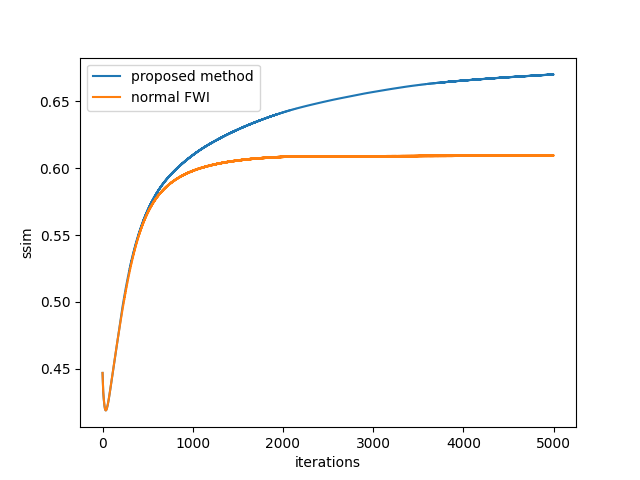
\includegraphics[width=80mm]{public/ssim}
    \caption{SSIM against the number of iterations.}
    \label{fig:ssim}
\end{center}
%\vspace{-\baselineskip}
\end{figure}

    \chapter{Conclusion}      \label{ch:conclusion}     In this paper, we developed an efficient algorithm to solve the TV and box constrained FWI problem% with neither inner loops nor approximations based on PDS. -> 後で書く
We demonstrated that the constrained problem can be fully handled within PDS.
We also demonstrated that the piecewise smoothness by the TV constraint is well represented, and that efficient and accurate reconstruction is possible.
%Furthermore, framework of PDS allows for the incorporation of more complex constraints and regularizations, making it a valuable tool for future research.


%inner loopとapproximationに触れる,

    \backmatter

    \chapter{Acknowledgment}  \label{ch:acknowledgment} \thanks{
    This work was supported in part by JST PRESTO under Grant JPMJPR21C4 and JST AdCORP under Grant JPMJKB2307, and in part by JSPS KAKENHI under Grant 22H03610, 22H00512, 23H01415, 23K17461, 24K03119, and 24K22291.
}

    %%%%%%%%%%%%%%%%%%%%%%%%%%%%%%%%%%%%%%%%%%%%%%%%%%

    \begin{spacing}{0.84}
%		\small
        \bibliographystyle{plain}
        \bibliography{references}
    \end{spacing}
\end{document}
